\usetikzlibrary{arrows.meta}
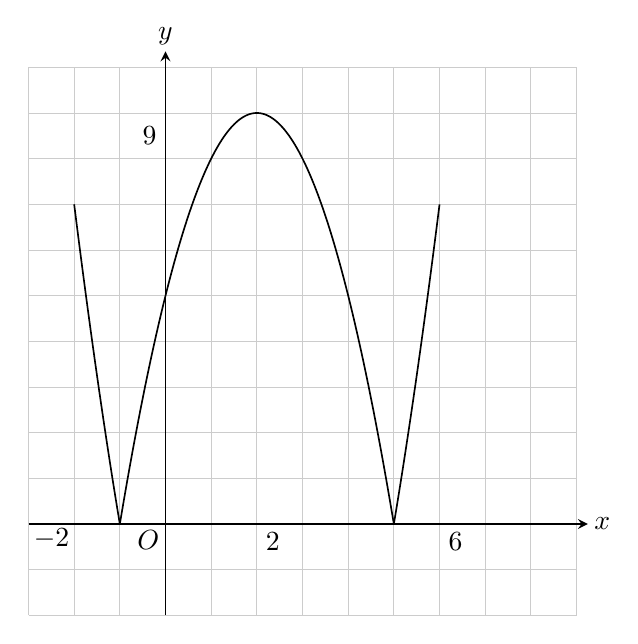
\begin{tikzpicture}[x=.58cm,y=.58cm,line width=.6pt,>=stealth]
\foreach \gx in {-3,...,9} \draw[gray!40,line width=.3pt] (\gx,-2)--(\gx,10);
\foreach \gy in {-2,...,10} \draw[gray!40,line width=.3pt] (-3,\gy)--(9,\gy);
\draw[->] (-3,0)--(9.25,0) node[right=2pt,inner sep=0pt] {$x$};
\draw[->] (0,-2)--(0,10.35) node[above=2pt,inner sep=0pt] {$y$};
\draw[domain=-2:-1,samples=61] plot (\x,{\x*\x-4*\x-5});
\draw[domain=-1:5,samples=181] plot (\x,{-\x*\x+4*\x+5});
\draw[domain=5:6,samples=61] plot (\x,{\x*\x-4*\x-5});
\node[below left,inner sep=0pt,xshift=-2pt,yshift=-2pt] at (0,0) {$O$};
\node[below left,inner sep=1.5pt] at (-2,0) {$-2$};
\node[below right,inner sep=0pt,xshift=3pt,yshift=-3pt] at (2,0) {$2$};
\node[below right,inner sep=0pt,xshift=3pt,yshift=-3pt] at (6,0) {$6$};
\node[left=3pt,inner sep=0pt,yshift=-8pt] at (0,9) {$9$};
\end{tikzpicture}
